We will now set up the Hartree-Fock equations by varying the coefficients of the single-particle functions.
The single-particle basis functions are defined as
\[
    \psi_p = \sum_{\lambda} C_{p\lambda} \psi_{\lambda}.
\]
where in our case $p=1,2,3,4$ and $\lambda = 1, 2, 3, 4$, that is the first four lowest single-particle orbits of Fig.~\ref{fig:schematic}.
Set up the Hartree-Fock equations for this system by varying the coefficients $C_{p\lambda}$ and solve them for values of $g \in [-1, 1]$.
Comment your results and compare with the exact solution.
Discuss also which diagrams in Fig.~\ref{fig:diagrams} that can be affected by a Hartree-Fock basis.
Compute the total ground state energy  using a Hartree-Fock basis and comment your results.

We will now study the system using non-degenerate Rayleigh-Schr\"odinger perturbation theory to third order in the interaction.
If we exclude the first order contribution, all possible diagrams (so-called anti-symmetric Goldstone diagrams) are shown in Fig.~\ref{fig:diagrams}.
\begin{figure}[hbtp]
    \centering
    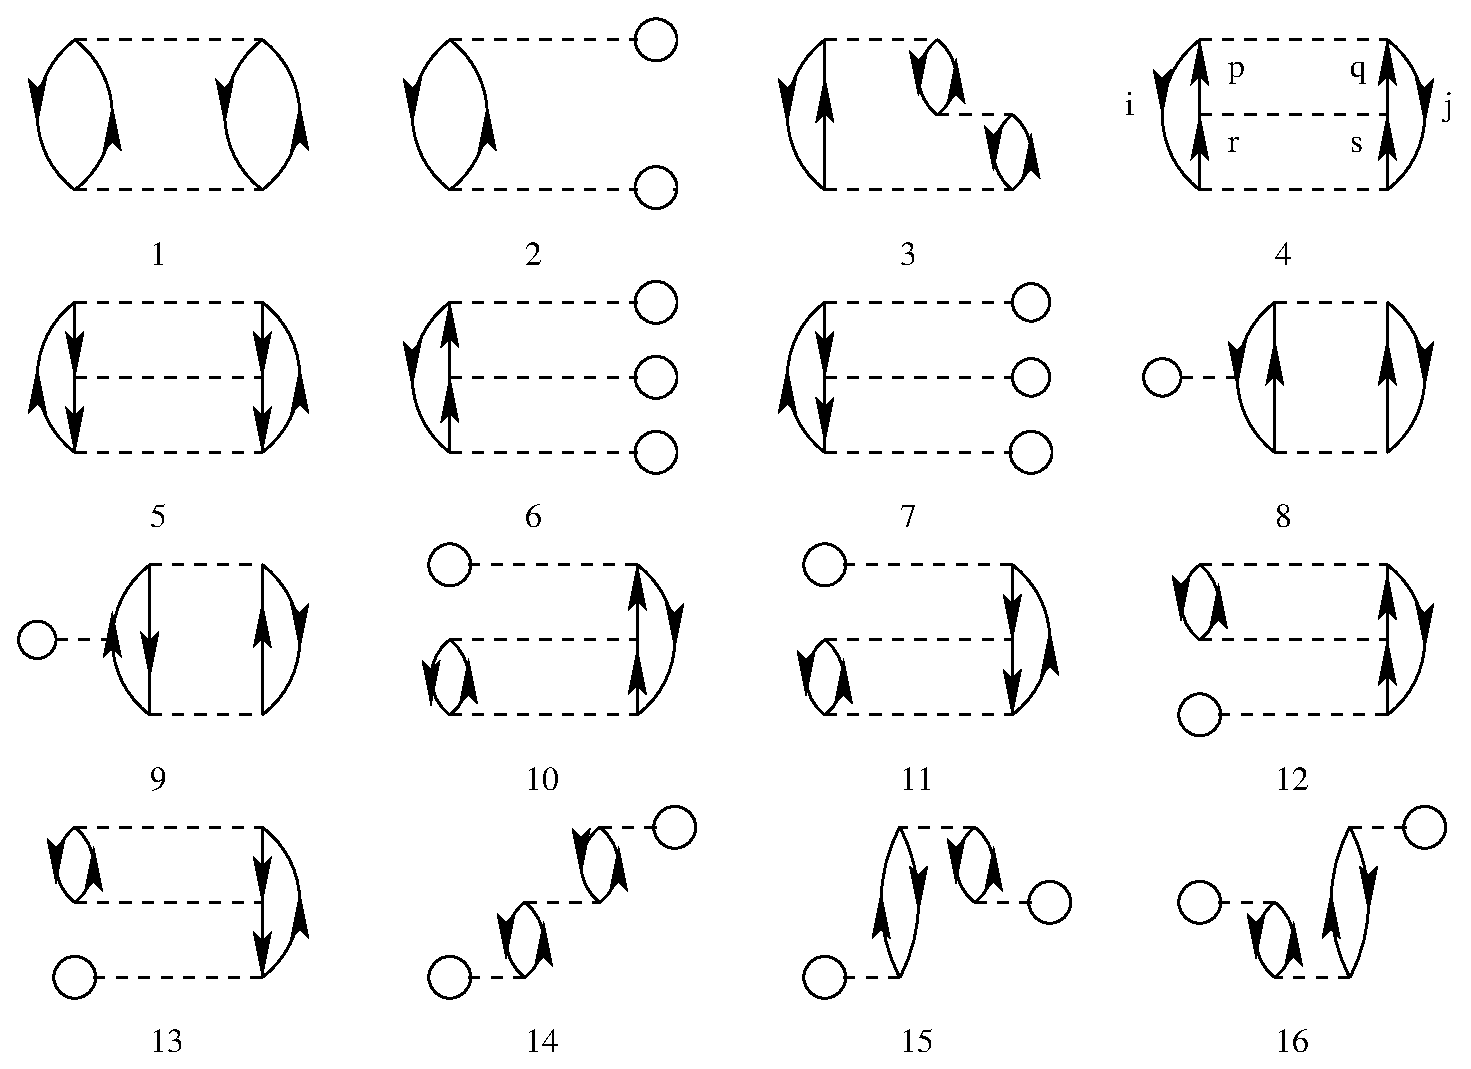
\includegraphics[width=.6\textwidth]{figures/diagrams.eps}
    \caption{
        Diagrams to third order in the interaction.
        The first order
        term is excluded.
        All interaction vertices represent anti-symmetrized matrix elements.\label{fig:diagrams}
    }
\end{figure}

Based on the form of the interaction, which diagrams contribute to the energy of the ground state?  Write down the expressions for the diagrams that contribute and find the contribution to the ground state energy as function $g\in [-1,1]$.
Comment your results.
Compare these results with those you obtained in 2) and 3). % chktex 9 % chktex 10 % tex-fmt: skip

\subsection{}
In the previous midterm, we found that the Hartree-Fock equations by way of varying coefficients are
\begin{equation*}
    \sum_{\gamma} h_{\alpha\gamma}^\HF C_{p\gamma} = \epsilon_p C_{p\alpha},
\end{equation*}
where the Hartree-Fock matrix elements are
\begin{equation*}
    h_{\alpha \gamma}^\HF = \expval{\alpha}{\hat{h}_0}{\gamma} + \sum_{\beta\delta} \rho_{\beta\delta} \expval{\alpha\beta}{V}{\gamma\delta}.
\end{equation*}

In order to simplify the calculations, we begin by computing the matrix elements of the one-body operator $\hat{h}_0$.
As computed previously, we have that
\begin{equation*}
    \expval{\alpha}{\hat{h}_0}{\gamma} = \delta_{\alpha\gamma} (\alpha - 1).
\end{equation*}
Next, we need to compute the matrix elements of the two-body operator $V$.
We require that the energy levels of bra and ket states match within, and that the spins of $\alpha$ and $\beta$ match those of $\gamma$ and $\delta$ respectively.

Writing $\bar{\alpha}$ as the quantum number with the same energy level as $\alpha$ but with opposite spin, we have that
\begin{align*}
    h_{\alpha\gamma}^\HF &= \delta_{\alpha\gamma} (\alpha - 1) + \rho_{\bar{\alpha}\bar{\gamma}} \expval{\alpha\bar{\alpha}}{V}{\gamma\bar{\gamma}} \\
    &= \delta_{\alpha\gamma} (\alpha - 1) - \rho_{\bar{\alpha}\bar{\gamma}} \frac{1}{2} g.
\end{align*}

We choose our initial guess for the coefficients to be the identity matrix, $C_{p\lambda} = \delta_{p\lambda}$, or equivalently $C = I \in \mathbb{C}^{8 \times 8}$.
We then solve the Hartree-Fock equations for $g \in [-1, 1]$.

Because of our initial guess for the coefficients, we have that the density function is
\begin{equation*}
    \rho = C^\dagger C = I^\dagger I = I.
\end{equation*}
This means that the Hartree-Fock matrix is initially entirely diagonal, with diagonal elements $\alpha - 1 - \frac{1}{2} g$.
As the matrix is diagonal, the eigenvalue problem is already solved.
We realized this after having implemented a solver, in the file \verb|src/hartree_fock.py|.

As the coefficients are the identity matrix, we have that
\begin{equation*}
    E[\Phi^\HF] = E[\Phi_0] = 2 - g.
\end{equation*}
plotted in Fig.~\ref{fig:hartree_fock_g}.

